\documentclass[a4paper,11pt]{article}
\usepackage{harvard}
\usepackage{setspace}
\usepackage{float}
\usepackage[margin=3cm]{geometry}
\usepackage{fontspec}
\usepackage{graphicx}
\setmainfont{Times-Roman}
\onehalfspacing


\begin{document}


\title{Internet of Things}
\author{Wangzhihui Mei \and Zijia He \and Xingjian Tian \and Miaojing Li \and Muzhe Peng \\ \\
Central China Normal Un \& 
University of Wollongong Joint-Institude}

\date{}
\maketitle
\thispagestyle{empty}
\clearpage


\newpage
\setcounter{page}{1} %Counting from this page

\section{Introduction}
The Internet of Thing (IoT) is seen as a major opportunity for development and change in the information field. As the government attaches great importance to the research and development of IoT, IoT has attracted great attention from Chinese academia, industry and news media, and the reports of IoT research and technology have become very popular\cite{dong2017understanding}.

The International Organization for Standardization/International Electrotechnical Commission (ISO/IEC) defines the IoTs as "an infrastructure of interconnected objects, people, systems and information resources, combined with intelligent services that enable them to process and respond to information from the physical and virtual worlds"\cite{iotdef}. In its earliest stages, the IoTs involves installing sensor devices for physical objects that need to be connected, enabling data collection, and then transmitting that data over a communications network to a data collection centre (e.g., a data management and analytics platform) to enable monitoring and analysis of that physical object, and ultimately to assist in rational decision-making. This traditional IoT information flow tends to be unidirectional, i.e., from the connected real Things to data collection centers. In recent years, the concept of the IoTs has been widely spread and applied in different industries, fostering a diverse range of IoT\cite{salman2018iot}. The smart home is the most common type of IoT. Unlike the early one-way flow of information, the smart home collects data on the operating status of electrical devices, and is able to give operating instructions to the corresponding devices to achieve real-time control of electrical equipment. This smart home as a representative of the IoTs to achieve the two-way flow of information, the integration of human or artificial intelligence analysis and control, improve the level of connected physical monitoring and management.

In general, IoT consists of different layers such as perception layer, access layer, network layer, management layer and application layer. The perception layer uses sensor elements or devices to provide information on the location and operating status of connected objects. the access layer connects sensors to the Internet, usually through radio frequency identification (RFID) communication, Bluetooth, Zigbee, WiFi, etc., and the network layer realizes extensive information integration. Exchange and Shared Internet platform, sometimes the access layer and network layer can be merged, management to achieve the management of information in the Internet, such as data storage, encryption, etc., application layer is through the integration and analysis of information, and ultimately provide appropriate services and make appropriate decisions. Still taking smart home as an example, smart switch, smart sensor and other devices are the perception layer, WiFi in the house is the access layer, wired/wireless Internet corresponds to the network layer, smart home corresponding mobile phone application (APP) may store the electricity consumption data of each electrical equipment, corresponding to the management, mobile phone APP through analysis or people through the APP, mobile phone APP is the access layer. This part controls the on/off of electrical equipment and the application layer.

\section{Features of the IoTs}
\subsection{Offline}
Objects in the IoTs have an extremely strong offline signature, which is due to a number of reasons. Technically speaking, the process is similar to Delay TolerantNetworks(DTN)\cite{vasilakos2016delay}, where objects have a distinct offline state. It can be seen that the offline state of the IoT is quite different from the offline state discussed in WsN because the offline state in the IoT is not caused only by congestion of the data link or node failure.

\subsection{Massive amount of devices}
As electronics, especially microelectromechanical systems (MEMS) technology, grows, the number of electronic devices grows, and IDC's John Gantz predicts that by 2015, 15 billion electronic devices will be interconnected over the Internet worldwide. Once the devices are connected to the Internet in various ways, how they are managed will make the already overburdened Internet even more challenging to manage. The assignment of UIDs (Unique IDs) to IoT devices is a fundamental technology for the interconnection of objects. Without UD, objects cannot be identified, nor can they be managed and maintained in a uniform manner.

\subsection{Massive amount of information}
The computing, storage and processing capabilities of IoT "objects" vary, ranging from simple RFID radio frequency cards to powerful video sensors. WSN is only used in small-scale applications where information processing can be divided into front-end and back-end processing. For IoT, with the increase of application scale and the increase of application types, distributed storage and distributed computing processing have become an urgent problem for IoT.

\subsection{Sematic operation}
The roadmap for the development of the IoTs published by EPoSS Europe states that semantic interoperability is one of the core elements of IoT research. This problem is also one of the most urgent problems of the Internet, which is referred to as "information islands" because of the difficulties of interoperability between different systems due to linguistic irregularities. The problem of semantic interoperability will become more and more obvious when the IoTs develops from the small-scale application of traditional WSN to large-scale application. For example, there is a temperature sensor in the IoT, which reports a temperature value by sensing the temperature. However, the temperature value is only a piece of data, and without additional semantic description, the value will not be available to other systems. This is the root cause of "information silos" in current WSN applications. International organizations have attempted to solve the problem of information interoperability by means of ontological knowledge expression, and a special working group has been established.



\section{Application of the IoTs}
The business and application layer is the information processing and application of the IoTs. It is oriented to various applications, realizing information storage, data mining, application decision-making, etc., involving intelligent processing of massive information, distributed computing, middleware, information discovery, etc. Kind of technology.

Since the network layer is composed of a variety of heterogeneous networks, and the applications of the IoTs are diverse, there is a need for middleware between the network layer and the application layer to connect the past and the next. Middleware is an independent system software or service program that can hide the complexity of the underlying network environment and deal with the heterogeneity between networks. Distributed application software uses middleware to share resources between different technologies. It is The key component of distributed computing and system integration\cite{1}. The article introduces the basic concepts of middleware, expounds a classification method based on the system level, and discusses in detail the characteristics, relevant standards and development applications of various existing middleware technologies. It has the function of simplifying the development of new services, and can combine various existing technologies into a new whole, so it is an indispensable part of the IoTs. In the past few years, middleware has adopted Service Oriented Architecture (SOA)\cite{3}. Services built on SOA can interact in a unified and universal way to achieve business Flexible expansion.

Cloud computing is the core element of IoT intelligent information analysis. The application of cloud computing technology makes it possible to manage hundreds of millions of various items in real time. With the development of IoTs applications and the increase in the number of terminals, cloud computing can be used to process massive amounts of information, make decision-making assistance, and improve the ability of IoTs information processing. Therefore, cloud computing, as a virtualized, hardware/software operational solution, can provide efficient computing and storage capabilities for the IoTs, and provide a network engine for the ubiquitous IoTs.

Judging from the current IoTs applications, each industry builds its own systems, which is not convenient for the expansion of multiple businesses. If there is no unified construction standard, standardized IoTs access, and integrated management platform, the IoTs will be due to the development of various industries. The difference cannot produce a scale effect, increasing the complexity and cost of use.

The above three-tier architecture is the general architecture of the IoTs that I believe. Among the existing research results, autonomous architecture\cite{2} and EPC \cite{4} are two representative IoT architectures, which are briefly introduced below.

Literature\cite{5} discusses an autonomous architecture of the IoTs, which is oriented to heterogeneous wireless communication environments and uses autonomous communication. The core of autonomous communication is selfware, which performs network control plane functions. The most important feature is to ensure the evolvability of the network, that is, the selfware can perform new functions of the network. The autonomous system of the IoTs is mainly composed of four types of planes: data plane, control plane, knowledge plane and management plane. The data plane transmits data, and the control plane sends configuration information to the data plane to optimize the throughput and reliability of the data plane. The knowledge plane contains information about the entire network and serves the adaptive control of the control plane, the management plane manages the data plane, control plane and The interaction of the knowledge plane.

EPC (Electronic Product Code) is a typical IoT application architecture.The EPC architecture is shown in the figure.
\begin{figure}[H]
\centering
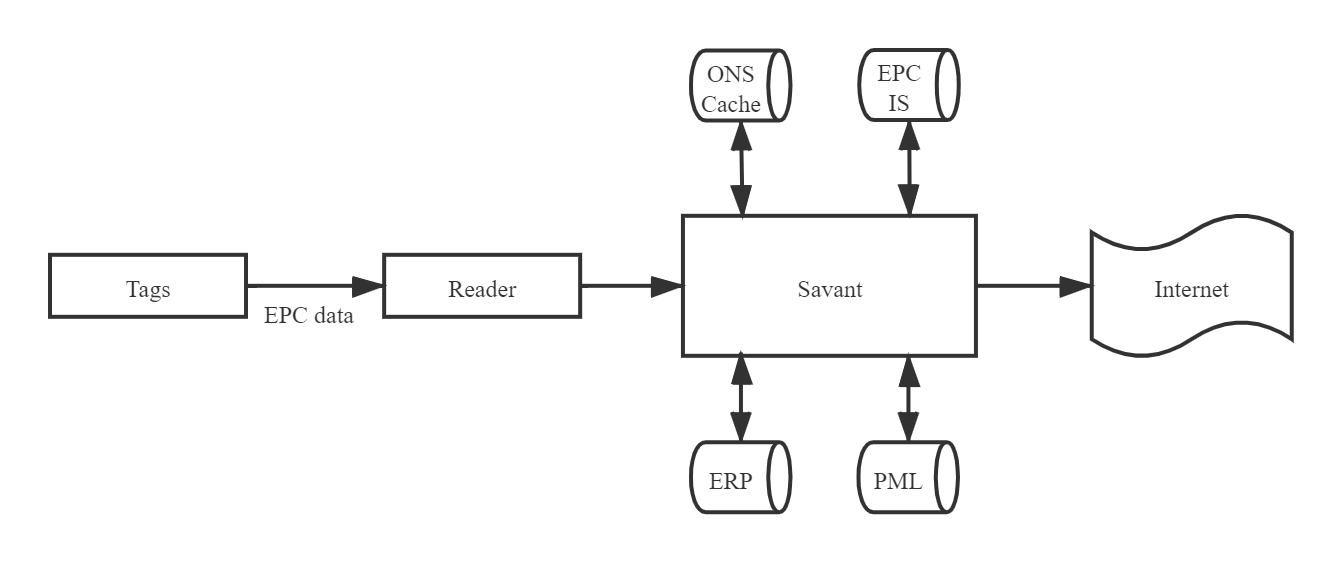
\includegraphics[width=6.5in]{figures/1.png}
\caption{The basic composition of EPC system}
\end{figure}
The EPC system structure involves EPC coding standards, EPC tags, readers, object name analysis services (Object Naming Serv.ice, ONS), Physical Markup Language (Physical Markup Lan.guage, PML) and so on. The EPC code encodes the object and its related information, thereby establishing a universal product electronic code. The product electronic code and other information of the object are stored on the EPC label, which is installed on the object. The reader reads the relevant information in the object tag by radio frequency, or writes relevant information into the tag. The object name resolution service matches the product electronic code to the corresponding product information, and its function is similar to the domain name resolution service (DNS) in the Internet. The physical markup language provides a general standard description language for remote monitoring and environmental monitoring of physical entities. EPC currently has important applications in logistics.
\section{Analysis of Key Technologies of IoTs}
In traditional research, sensor technology and identification technology are separated. For example, RFID is used to identify a specific object, and sensor technology is used to perceive the physical state of this object. The intelligent identification and perception technology in the IoTs must integrate identification technology and sensing technology.

As a research hotspot in the field of information science and computer network, the IoTs has the characteristics of interdisciplinary and multi-technology integration. Each key technology needs to be broken through\cite{6}. The key technologies of the IoTs can be from the hardware Consider the two aspects of software and software. Hardware technology includes radio frequency identification technology (RFID), wireless sensor network technology (WSNs), intelligent embedded technology (Embedded Intelligence) and nanotechnology (Nanotechnology), software technology includes information processing technology, self-organization management Technology, safety technology.

Intelligent identification and perception technologies for specific types of applications show differences. For example, when acquiring the identification and status of the container, it is necessary to use anti-interference active electronic tags to obtain the status of the user's interest, such as the temperature in the box, the opening and closing status of the door, etc. Different, the amount of state that users are interested in is also different.
\subsection{Hardware technical analysis}
By defining the following three abstract concepts, the role of key technologies in IoT hardware can be further explained.
\begin{enumerate}
    \item Object: Any thing in the objective world can be regarded as an object, and tens of thousands of objects prove the existence of the objective world. Each object has two characteristics: attributes and behaviors, and attributes describe the static state of the object Feature, behavior describes the dynamic characteristics of an object. Any object is often composed of a set of attributes and a set of behaviors.
    \item Message: A message sent by the objective world to the object. The existence of the message indicates that the object can respond to external stimuli in the objective world. Each object can transmit and exchange information through messages.
    \item Encapsulation: Integrate related attributes and behaviors into an object to form a basic unit.
\end{enumerate}


The relationship between the three is shown in the figure.
\begin{figure}[H]
\centering
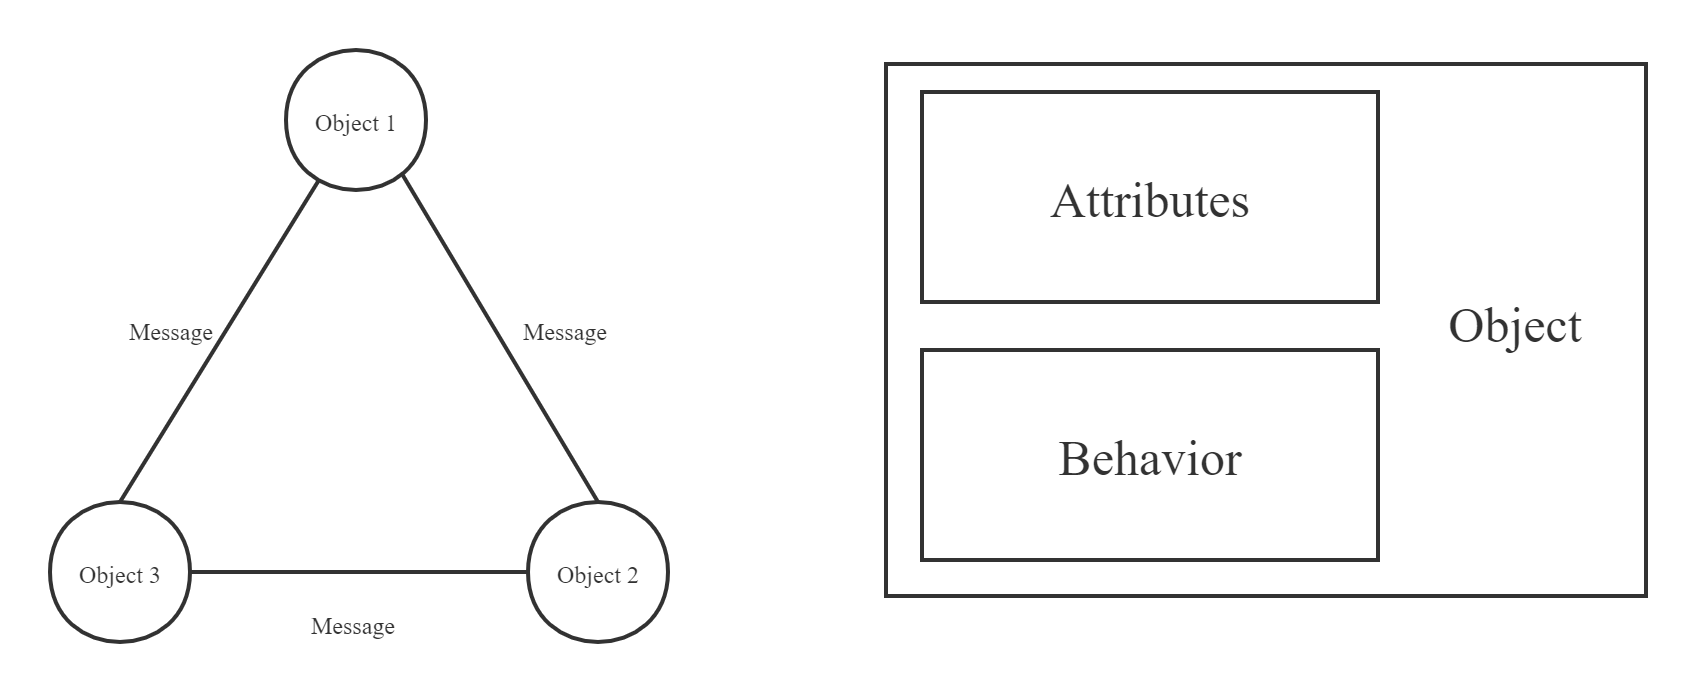
\includegraphics[width=6.5in]{figures/2.png}
\caption{Object relationship diagram}
\end{figure}
One of the important features of the IoTs is to enable the exchange of information between objects, and each object is an object. Therefore, the key hardware technology of the IoTs must be able to reflect the characteristics of each object. First, RFID technology\cite{7} uses The radio frequency signal identifies the target object and reads the object.This information reflects the characteristics of the object itself and describes the static characteristics of the object. Secondly, in addition to identifying the static characteristics of the object, for each object in the IoTs, the ability to detect changes in their physical state and record Their dynamic characteristics in the environment need to be considered.In this regard, sensor networks play an important role in bridging the gap between the physical and virtual worlds. It describes the dynamic characteristics of objects. Again, the intelligent embedding technology works by implanting each independent node in the IoTs After the embedded chip, it has more powerful intelligent processing and data transmission capabilities than ordinary nodes. Each node can process and respond to external messages (stimuli) through intelligent embedded technology. At the same time, nodes with intelligent embedded technology can make The processing power of the entire network is allocated to the edge of the network, which increases the flexibility of the network. Finally, the progress of nanotechnology and miniaturization means that smaller and smaller objects will have the ability to interact and connect and effectively encapsulate\cite{8}. However, the development of existing nanotechnology will theoretically bring the line width of semiconductor devices and integrated circuits to the limit. This is because if the line width of the circuit continues to become smaller, the insulating film constituting the circuit will become more and more Thin, this will destroy the insulation effect of the circuit, which will cause the problem of circuit heating and jitter.
\subsection{Software technical analysis}
The software technology of the IoTs is used to control the working methods and working behaviors of the underlying network distribution hardware, and provide a reliable operation platform for the design of various algorithms and protocols. On this basis, it is convenient for users to effectively manage the IoTs and realize the IoTs Information processing, security, service quality optimization, etc.
Functions to reduce the complexity of using the IoTs for users.

As mentioned earlier, IoT hardware technology is the basis for the design of embedded hardware platforms. The board-level support package is equivalent to the hardware abstraction layer, located on the embedded hardware platform, used to separate the hardware and provide a unified hardware interface for the system. The kernel is responsible for the scheduling and distribution of processes, and the device driver is responsible for driving the hardware devices, and they jointly provide an interface for the data control layer. The data control layer implements software support technology and communication protocol stacks, and is responsible for coordinating the sending and receiving of data. The program needs to be designed according to the interface provided by the data control layer and related global variables.

The IoTs software technology describes the tasks and required services of the entire network application. At the same time, through the software design, it provides an operating platform for users to manage the network and verify the evaluation environment. Each node of the network delivers services through the connection of middleware. The cloud computing information processing technology, self-organizing management technology, and security technology in the middleware exist logically in the network layer, but physically exist inside the node, and coordinate task management and resource allocation within the network, and perform mutual interactions between multiple services operation.
\section{Conclusion}
The development of the IoTs currently presents a different approach from the development of the Internet. It is manifested as being driven by partial and closed-loop applications, and gradually forming an open and global framework of the IoTs. In the future of audio applications, it will develop from a single object identification technology to an intelligent executive body integrating object identification, sensing, control and execution. The IoTs will eventually be the question of intelligent, intelligent and non-intelligent. A globally integrated network for related communications and information sharing. This article describes the concept, architecture, core technology, open research issues, and application evolution trends of the IoTs. At present, the theories, methods, and core technologies of the open IoTs are still in the research stage, and closed-loop IoTs applications can be implemented on a local scale, but it will inevitably bring standards and methods to the Internet from the closed loop. In the process of continuous evolution to open loop, in order to avoid the repeated construction and waste of resources, it is necessary to take into account the special requirements of specific applications and the common technical characteristics of applications in various industries, and formulate unified standards for public applications.



\clearpage
\bibliographystyle{agsm}
\bibliography{wpref}
\end{document}